\chapter{CMS Computing and Offline}
\label{c:CMS_computing_and_offline}

\section{CMS Computing}
\label{s:CMS_computing}

The CMS offline computing infrastructure takes on the workload of transferring accepted data from the triggers
to both permanent and temporary storage, of processing this data for subsequent analysis, in addition to the
production of simulated CMS data. The resources needed to process the high volumes of data involved require a
distributed computing system. The Worldwide LHC Computing Grid (WLCG) infrastructure, an international
collaboration of LHC experiments and computing centres, is employed to carry out these tasks.

CMS computing resources are primarily divided into three tiers. Tier 0 (T0) consists of only one site, at CERN
itself. The T0 centre has as its main aim to take accepted data from the detector and transfer it to permanent
storage on tape. Tier 0 computing is also responsible for reconstructing the initial RAW data into smaller
formats, by passing events through modules to produce physics objects (like electrons and jets) using
algorithms to reconstruct tracks in the silicon tracker, clusters of deposits in the calorimeters, primary and
secondary vertices, determine particle identification and to correct for detector characteristics such as
non-functioning components (see Section~\ref{s:Event_Data_Model} onwards for more details on data formats).
From the T0 centre, copies of the data in RECO and RAW format are transferred to T1 centres around the world.
Owing to its crucial role in ensuring the reliable transfer of RAW and RECO data, T0 resources are not
available for analysis by CMS users. There are seven Tier 1 centres located in various countries within the
CMS collaboration. The UK T1 centre is located at the Rutherford Appleton Laboratory in Harwell, near Oxford.
T1 centres provide reliable computing resources for data storage and processing. RAW data is spread between
them, providing a second copy of the RAW data stored at CERN. The second reconstruction step, termed RERECO,
is also carried out at T1 centres, in addition to the production of simulated data. These can then be provided
to any of the Tier 2 centres at CMS institutes (typically universities) where they may be temporarily stored.
T2 centres are also generally used to run users' final analyses and produce simulations
\cite{CMS_experiment,CMS_TDR1}.

\section{Event Data Model}
\label{s:Event_Data_Model}
Reconstructed data from CMS uses a data model based around an event, called the Event Data Model (EDM), where
one event is one crossing of proton bunches at the centre of CMS that passes the triggers. This model
is created and manipulated within a CMS software framework (CMSSW)~\cite{cmssw} written in C++, with the event
and related objects in the object-oriented data analysis framework ROOT~\cite{ROOT}.

The iterations of data from the initial recorded information to subsequent, more compact formats, are produced
by passing events through a sequence of modules. The arrangement of these data takes the form of several
layers, with the first of these being RAW. This level contains the full information from the event in CMS and
occupies approximately 1.5-2~MB/event. More information than is necessary for user analyses is included at
this level, and so the majority of CMS users will not use this data format. Reconstructed level data (RECO) is
slightly smaller in size (approximately 0.5~MB/event) and is essentially a compressed subset of the RAW data
after modules performing reconstruction have been run.

The third level, Analysis Object Data (AOD), is the smallest of the data formats, requiring approximately
100~kB/event, which is small enough to allow the entire AOD data to be stored at computing centres worldwide.
AOD format is a subset of the RECO data, and is produced by further reducing RECO, leaving only high level
physics objects (e.g. electrons, jets) which is adequate for most physics analyses. 

In the differential cross section analysis presented in this thesis, this AOD data is processed using the
Bristol Top Group's NTupleProduction code~\cite{NTT_LukeKreczko_SergeySenkin_JesonJacob_EmyrClement_2015} to
produce private ntuples which are yet again smaller in size, at approximately 3~kB/event. These ntuples are
then converted to simple ROOT histogram files after applying the required selection criteria and corrections
in the BristolAnalysisTools~\cite{BAT_LukeKreczko_JesonJacob_SergeySenkin_EmyrClement_2015}. Scripts written
in Python in DailyPythonScripts~\cite{DPS_LukeKreczko_SergeySenkin_JesonJacob_EmyrClement_2015} are then used
to produce final results plots and tables.


\section{Object Reconstruction and Identification}
\label{s:object_reconstruction_and_identification}

The process of producing a physics object such as an electron, photon or jet, from the data recorded by CMS is
known as reconstruction and is carried out by modules qknown as EDProducers within CMSSW. The three-step
process of reconstructing high level objects consists of local reconstruction within a sub detector, global
reconstruction using data from the whole CMS detector, and a final stage combining reconstructed objects from
the first two stages. The reconstruction technique used in the majority of CMS analyses is called Particle
Flow (PF) \cite{particle_flow}. PF uses information from all of the sub-detectors of CMS to identify and reconstruct
particles produced from a proton-proton collision.

\subsection{Track Reconstruction}
\label{ss:track_reconstruction}
Algorithms performing local track reconstruction execute a scan to identify tracker modules that receive a
higher than threshold signal. Clusters are then constructed by adding adjacent strips or pixels to the
originally identified seed strip or pixel. In order to reconstruct complete tracks to obtain the position and
momentum of the charged particle, algorithms based on specific requirements such as high or low transverse
momentum tracks are used. These algorithms in CMS are collectively known as the Combinatorial Track Finder
(CTF).

Multiple passes of the CTF reconstruction software are carried out to reconstruct tracks, in a process called
iterative tracking. The earliest iterations identify tracks that are easy to find such as high \pt tracks
originating near the interaction point. As these tracks are reconstructed, the corresponding hits are removed
from consideration in subsequent iterations, making it simpler for later iterations to identify tracks that
are more difficult to find such as those of displaced particles or with low \pt.

Six iterations are carried out in total, and each iteration can be split into four steps. Seeds are created
using 2 or 3 hits to produce intial track candidates. The seed gives an estimate of the trajectories of the
potential track candidates. A Kalman Filter \cite{kalman_filter, Speer:927395} based track finding algorithm
then looks for further hits along an extrapolated path of the seed trajectory. A track fitter is then run
using information from the previous steps to produce final values for trajectory parameters. The fourth and
final step then rejects tracks which fail specified quality checks \cite{track_reconstruction}.

\subsection{Pileup Subtraction}
\label{ss:pileup_subtraction}
When reconstructing an event in CMS, all vertices (points from which multiple tracks originate) in the event
must be reconstructed. By ordering the vertices by the sum of the transverse momenta of their tracks, it is
possible to identify the the vertex of interest for physics analyses, known as the primary vertex (PV), as the
vertex with the largest transverse momentum. The particle flow algorithm reconstructs objects, starting with
those coming from the primary vertex, followed by other vertices (known as pileup). The reconstructed objects
from the PV can be affected by the number of other vertices present in the event. For example, the jet
momentum and lepton isolation could both increase with high pileup. This can, in turn, lead to signal events
not passing selection requirements because a truly isolated lepton from the PV may appear not to be isolated.
In addition, a larger number of events from background processes may pass selection requirements due to low
energy jets appearing to have a higher energy. Hence, pileup subtraction, the removal of charged particles
coming from vertices other than the PV is implemented to reduce these effects.

Neutral particles, however, pose a more difficult problem since they leave no tracker information for the
reconstruction algorithms to easily identify their origin. One method of removing such particles from an
event, known as the $\Delta\beta$ correction, uses the fact that the estimated average energy in an event from
neutral particles is half that from charged particles. Thus, it can be estimated that 0.5 times the charged
particle energy comes from neutral particles. The second method, known as $\rho$ correction, subtracts an
average transverse momentum coming from pileup per unit area. While the two methods produce similar results,
the $\rho$ correction is used to correct the electron isolation and the $\Delta\beta$ correction is used to
correct the muon isolation in the differential cross sections analysis presented in this thesis, as
recommended by the CMS TOP physics analysis group.

\subsection{Electron Reconstruction}
\label{ss:electron_reconstruction}
ECAL local reconstruction algorithms calculate the time of arrival, position and the energy of deposits. After
grouping together deposits in neighbouring crystals to form clusters, deposits are then matched to deposits in
the HCAL, forming a Calo Tower. Electrons are, typically, completely stopped in the ECAL and deposit their
energy in a narrow cluster of crystals.

However, electrons can interact with the material between the interaction point and the ECAL, emitting a
photon via bremsstrahlung radation. Similarly, photons can convert to an elecron-positron pair ($e^{+}e^{-}$).
Both of these processes result in ECAL deposits with a larger spread in $\phi$ because of the strong magnetic
field in the inner section of CMS containing the tracker. In the case of photons, several clusters are grouped
together to form superclusters, which are then corrected for their energies to obtain the energies of the
original photon \cite{photon_reconstruction}.

Electron reconstruction in the ECAL is carried out by two methods. The first matches superclusters with a
trajectory compatible with two or three pixel detector hits and the interaction point. The second matches the
supercluster to tracker tracks to identify electrons (and in the case of electrons emitting bremsstrahlung
radiation, tracks with a low number of hits) \cite{electron_reconstruction}. Combining the seeds from the two
methods, a Gaussian-Sum Filter, a generalisation of the Kalman Filter algorithm, is used to reconstruct
electron paths \cite{electrons_GSF}.

Since other objects can leave similar signatures in the detector to electrons, such as jets or electrons from
photon conversions, candidates are required to satisfy additional requirements of identification and
isolation. Several electron identification methods exist and are used in CMS analyses. The top cross sections
analysis in this thesis uses the multivariate identification (MVA ID). As the name suggests, this approach
uses a multivariate analysis, with track, track quality, and supercluster variables as input, to produce a
discriminator value, with higher values indicating a higher likelihood for a candidate to be a real electron.
The MVA ID algorithm is optimised for identifying electrons from W and Z boson decays, and separately for
triggering and non-triggering electrons~\cite{electron_reconstruction}.

The isolation of an electron is defined as the activity within a cone surrounding the electron. Isolation is
used as an additional criterion to select electrons, in particular to distinguish electrons promptly produced
in a proton-proton collision. Such isolated electrons would have less activity in its vicinity than electrons
from within a jet, which could originate from leptonically decaying b hadrons, and jets faking electrons. Two
methods exist in CMS of calculating the isolation of a particle: detector based isolation and particle based
isolation. The detector based method is defined in each sub detector as the sum of the momenta or energies in
a cone of $\Delta R = 0.3$ around the electron. The particle based method uses the total transverse energy of
PF reconstructed particles within a cone of $\Delta R = 0.3$ and can remove activity coming from collisions
other than the hard proton-proton interaction of interest. By normalising this isolation to the momentum or
energy of the electron, a relative isolation is obtained, relating the cone activity to the electron.
Termed PFRelIso, it is this relative isolation that is used in the cross section analysis to select
electrons.
% can improve signal efficiency

In order to avoid the selection of electrons originating from a photon conversion, a veto can be placed on a
second electron in the event. However, since the two electrons in a photon conversion may not necessarily have
equal transverse momentum, \ie one may have a very low \pt, such a veto may be insufficient, and so further
techniques to identify conversion events are used. Firstly, since an electron from a conversion would be
produced at some distance from the interaction point and in the detector material, eliminating candidates with
missings hits in the pixel tracker helps to distinguish such electrons from promptly produced electrons. In
events in which the conversion occurs in the beam pipe or if the electron is matched to unassociated pixel
hits, this method can also be insufficient, so an additional track matching step is used. Tracks are matched
in pairs and following geometrical cuts, can be removed if they appear to originate from a conversion
\cite{electron_reconstruction}.

\subsection{Muon Reconstruction}
\label{ss:muon_reconstruction}
Local reconstruction in the muon chambers provides hit position and time of arrival of a muon. This
information from the DTs and CSCs is then amalgamated to create muon track hits and segments, which are then
used by the muon global reconstruction algorithms to reconstruct ``standalone'' muons. An inner detector
segment is used as a seed for a Kalman Filter~\cite{kalman_filter, Speer:927395} and possible trajectories are
generated. By removing hits which are unlikely to have come from the track in question, the likely trajectory
is constructed layer-by-layer. A final fit is carried out, including an extrapolation to the interaction point
for greater momentum resolution.

Muons are also independently reconstructed in the tracker. These tracker tracks can therefore be combined with
the aforementioned muon chamber information, where the magnetic field is only 2~\tesla, to improve the \pt
resolution of muons, as seen in Figure~\ref{fig:muon_momentum_resolution}.

\begin{figure}[hbtp]
   \centering
     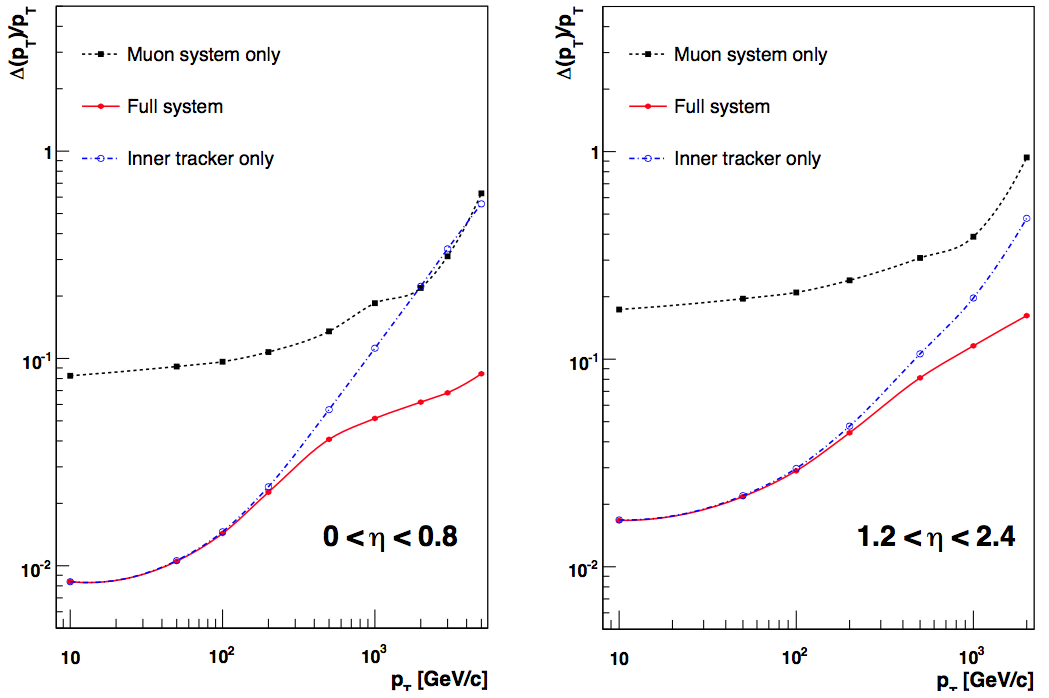
\includegraphics[width=0.65\textwidth]{Chapters/02_Detector/Images/muon_momentum_resolution.png}\hfill
     \caption[Muon transverse momentum resolution using muon system and the tracking system.]{Muon transverse
     momentum resolution as a function of muon transverse momentum using the muon system only, using inner tracking only,
     and using both~\cite{Chatrchyan:2012xdj}.}
     \label{fig:muon_momentum_resolution}
\end{figure}

Two methods are employed to combine the information from the two sub-detectors. \textit{Global muon
reconstruction} matches a tracker track to a standalone muon track and carries out a fit of the resulting
\textit{global muon} track. The second method, \textit{tracker muon reconstruction}, extrapolates tracker
tracks outwards to the muon chambers and accepts a muon candidate if a DT or CSC matching track is found and
the muon \pt is greater than 0.5\GeV~\cite{muon_reconstruction}.

For triggering, the \pt of a muon is first estimated using the information available at Level 1 from all three
types of muon detectors. At HLT level, the muon candidates from Level 1 are further refined using track
finding and fitting, but still using only information from muon chambers, leading to Level 2 muons. As
mentioned in Section~\ref{ss:Trigger}, due to the time constraints required of the L1 trigger, full tracker
data are not currently used. However, tracks of Level 2 muons are extrapolated into the tracker systems and a
localised track finding algorithm is run to identify only nearby tracker hits. A track matching that of a
Level 2 muon leads to a Level 3 muon. %See Emyr's thesis P45 top for details.

\subsection{Jet Reconstruction}
\label{ss:jet_reconstruction}
As quarks produced in proton-proton interactions (except the top quark) hadronise~\cite{Griffiths:1987tj},
jets of particles are formed in the direction of travel of the quark. The time of arrival, position and the
energy deposited by hadronic objects are locally reconstructed in the HCAL. If the deposit matches an ECAL
deposit, a Calo Tower is formed for later use in jet reconstruction algorithms.

The PF algorithm performs the reconstruction of particles in the jet, and the \antikt algorithm is used to
perform the clustering of these particles into jets. The \antikt algorithm, explained in detail
in~\cite{Cacciari:2008gp}, is one of several jet algorithms that exist in CMS to combine reconstructed
particles into jets. It defines a distance $d_{ij}$ between reconstructed particles as
\begin{equation}
%\begin{center}
d_{ij} =
min\left(\frac{1}{p_{T,i}^{2}},\frac{1}{p_{T,j}^{2}}\right)\frac{(\eta_{i}-\eta_{j})+(\phi_{i}-\phi_{j})^{2}}{R^{2}}.
%\end{center}
\end{equation}
$p_{T,i}$ and $p_{T,j}$ are the transverse momenta of the two particles $i$ and $j$, $\eta_{i}$ and $\eta_{j}$
are the rapidities, $\phi_{i}$ and $\phi_{j}$ are the azimuth angles and $R$ is the radius of the jet cone.
The \antikt algorithm iteratively clusters together particles with the smallest $d_{i,j}$ between them until
all jets are reconstructed and there are no particles remaining. Events will usually consist of a small number of
high-\pt (hard) particles and a large number of low-\pt (soft) particles. The distance between hard particles
is typically small, and the distance between softer particles is larger. Soft particles tend to
cluster around hard particles first, before clustering with other soft particles.

While the PF anti-$k_{t}$ jets show high jet matching efficiency on Monte Carlo simulation samples,
corrections are applied based on the jet $\pt$ and $\eta$ to correct for mismeasurements in the
detector and thereby improve the agreement between generated and reconstructed particle flow jets. The
factored approach to CMS jet energy corrections is comprised of three parts:
\begin{enumerate}
  \item {L1 Pile Up: corrects for additional energy from charged particles from pile-up in the event
  \ref{ss:pileup_subtraction}.}
  \item {L2 Relative Jet Correction: corrects the reconstructed energy to match the generated jet with respect
  to $\eta$.} %to flatten the jet response in the ecal eta
  \item {L3 Absolute Jet Correction: corrects the reconstructed energy to match the generated jet with respect
  to $\pt$.} %to flatten the jet response in the ecal pt
  \item {L2L3Residuals: reduces any residual differences between the reconstructed and generated
  jet due to simulation not being perfectly tuned to data. This correction is applied to data only.}
  %https://twiki.cern.ch/twiki/bin/viewauth/CMS/IntroToJEC
\end{enumerate}
In order to identify jets in the differential cross sections analysis, further identification criteria are
used to reduce electronic noise, to reduce the number of electrons mis-identified as jets and, in so doing, to
ensure the selection of high quality jets. The requirements, which are known as the loose PF Jet ID, are:

\begin{itemize}
  \item at least one constituent particle
  \item the neutral hadron energy fraction (NHF) must be $<0.99$
  \item for jets with \abseta$<2.4$, the charged hadron energy fraction (CHF) must be $>0$
  \item the neutral electronmagnetic energy fraction (NEF) must be $<0.99$
  \item for jets with \abseta$<2.4$, the charged electronmagnetic energy faction (CEF) must be $<0.99$
  \item for jets with \abseta$<2.4$, the number of charged hadronic constituents (NCH) must be $>0$
\end{itemize}

\subsubsection{B Jets}
\label{sss:b_jets}
The process of identifying jets coming from \bquarks is known as \btagging and is very important in top quark
physics due to the decay of the top to a \W boson and a \bquark. Effective \btagging can therefore help to
appreciably reduce background processes in an analysis. A description of \btagging, the several algorithms
available in CMS, relevant event variables, and a performance comparison, is given in
Chapter~\ref{c:b_tagging_study}.
